\documentclass[a4paper,11pt]{article}
\input{/home/tof/Documents/Cozy/latex-include/preambule_lua.tex}
\newcommand{\showprof}{show them}  % comment this line if you don't want to see todo environment
\fancyhead[L]{Représentation des entiers naturels}
\newdate{madate}{10}{09}{2020}
\fancyhead[R]{Première - NSI} %\today
\fancyfoot[L]{~\\Christophe Viroulaud}
\fancyfoot[C]{\textbf{Page \thepage}}
\fancyfoot[R]{\includegraphics[width=2cm,align=t]{/home/tof/Documents/Cozy/latex-include/cc.png}}
\usepackage{tikz}

\begin{document}
\begin{Form}
\section{Problématique}
Dans un ordinateur l'UAL du microprocesseur réalise les opérations arithmétiques. Pourtant nous savons qu'il n'est composé que de transistors qui laissent ou non passer le courant. Ce comportement \emph{binaire} est la base de l'information dans la machine.
\begin{center}
\shadowbox{\parbox{14cm}{\centering Comment alors représenter les nombres entiers dans la mémoire de l'ordinateur?}}
\end{center}
\section{Cellules mémoires}
Le passage du courant ou non est représenté par les chiffres 0 ou 1. Nous parlons de \textbf{BInary DigiTS} ou plus simplement la contraction \textbf{bits}. 
\begin{figure}[!h]
\centering
\begin{tikzpicture}[scale=0.5]
\draw (0,0) -- (1,0) ;
\draw (1,0) -- (1,1) ;
\draw (1,1) -- (0,1) ;
\draw (0,1) -- (0,0) ;
\end{tikzpicture}
\captionof{figure}{1 bit}
\end{figure}

Dans la mémoire d'un ordinateur, ces chiffres sont regroupés par paquet de huit qu'on appelle \textbf{octet} (ou \textbf{bytes} en anglais).
\begin{figure}[!h]
\centering
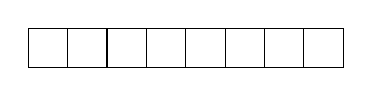
\begin{tikzpicture}[scale=0.5]
\draw (0,0) -- (8,0) ;
\draw (8,0) -- (8,1) ;
\draw (8,1) -- (0,1) ;
\draw (0,1) -- (0,0) ;

\draw (1,0) -- (1,1) ;
\draw (2,0) -- (2,1) ;
\draw (3,0) -- (3,1) ;
\draw (4,0) -- (4,1) ;
\draw (5,0) -- (5,1) ;
\draw (6,0) -- (6,1) ;
\draw (7,0) -- (7,1) ;
\end{tikzpicture}
\captionof{figure}{1 octet}
\end{figure}
Les octets sont organisés en \emph{mots machines} de 2, 4 ou 8 octets. Une machine \emph{32 bits} manipule des mots de 4 octets (4×8 = 32 bits) lorsqu'elle effectue des opérations.
\begin{figure}[!h]
\centering
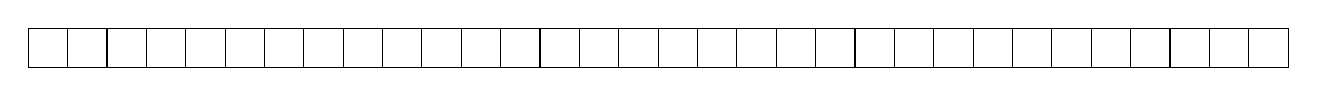
\begin{tikzpicture}[scale=0.5]
\draw (0,0) -- (32,0) ;
\draw (32,0) -- (32,1) ;
\draw (32,1) -- (0,1) ;
\draw (0,1) -- (0,0) ;

\draw (1,0) -- (1,1) ;
\draw (2,0) -- (2,1) ;
\draw (3,0) -- (3,1) ;
\draw (4,0) -- (4,1) ;
\draw (5,0) -- (5,1) ;
\draw (6,0) -- (6,1) ;
\draw (7,0) -- (7,1) ;
\draw (8,0) -- (8,1) ;
\draw (9,0) -- (9,1) ;
\draw (10,0) -- (10,1) ;
\draw (11,0) -- (11,1) ;
\draw (12,0) -- (12,1) ;
\draw (13,0) -- (13,1) ;
\draw (14,0) -- (14,1) ;
\draw (15,0) -- (15,1) ;
\draw (16,0) -- (16,1) ;
\draw (17,0) -- (17,1) ;
\draw (18,0) -- (18,1) ;
\draw (19,0) -- (19,1) ;
\draw (20,0) -- (20,1) ;
\draw (21,0) -- (21,1) ;
\draw (22,0) -- (22,1) ;
\draw (23,0) -- (23,1) ;
\draw (24,0) -- (24,1) ;
\draw (25,0) -- (25,1) ;
\draw (26,0) -- (26,1) ;
\draw (27,0) -- (27,1) ;
\draw (28,0) -- (28,1) ;
\draw (29,0) -- (29,1) ;
\draw (30,0) -- (30,1) ;
\draw (31,0) -- (31,1) ;
\end{tikzpicture}
\captionof{figure}{1 mot-machine 32 bits}
\end{figure}
\begin{activite}
Chaque bit accepte 2 valeurs possibles: 0 ou 1. Avec 1 bit nous pouvons donc avoir 2 combinaisons possibles.
\begin{enumerate}
\item Combien de combinaisons peut-on réaliser avec 1 octet?
\item Même question pour 1 mot-mémoire 32 bits?
\end{enumerate}
\end{activite}
\section{Encodage des entiers naturels}
Afin de représenter un entier naturel en mémoire, il suffit de le convertir en base 2.
\subsection{Écriture en base 10}
Le principe de l'encodage en base 2 s'appuie sur le même modèle que celui en base 10. Rappelons ce principe:
$$6103 = 6×10^3 + 1×10^2 + 0×10^1 + 3×10^0$$
\begin{activite}
\begin{enumerate}
\item Décomposer 76035 en base 10.
\item Combien d'entiers en base 10 peut-on représenter avec 4 chiffres? Indiquer le plus petit et le plus grand.
\item Combien d'entiers en base 10 peut-on représenter avec \emph{k} chiffres? Indiquer le plus petit et le plus grand.
\end{enumerate}
\end{activite}
\subsection{Écriture en base 2}
Afin d'éviter les ambiguïtés il est possible d'écrire un nombre en précisant sa base: $1001_2$.
\begin{activite}
\begin{enumerate}
\item En s'appuyant sur le principe du paragraphe précédent, calculer la valeur de l'entier du nombre binaire suivant: $101101_2$.
\item Écrire en base 2 les entiers de 0 à 10.
\item Combien d'entiers peut-on représenter avec 8 chiffres binaires (\emph{soit 1 octet)}? Indiquer le plus petit et le plus grand.
\item Combien d'entiers peut-on représenter avec \emph{k} chiffres binaires? Indiquer le plus petit et le plus grand.
\item Quel est le plus grand entier que l'on peut stocker dans un mot-mémoire 32 bits?
\end{enumerate}
\end{activite}
\subsection{Unités de mesures}
Comme pour les unités de masse, de longueur, il est pratique de convertir la capacité mémoire d'un ordinateur.
\begin{center}
1 kilooctet = 1000 octets
\end{center}
\begin{activite}
\begin{enumerate}
\item En s'aidant de la page Wikipedia: \url{https://fr.wikipedia.org/wiki/Octet#Multiples_normalis.C3.A9s}, citer les principaux multiples utilisés dans la vie quotidienne.
\item Associer chaque mémoire à un multiple de l'octet: disque dur, barette RAM, registre du processeur, clé USB, DVD.
\item Bob achète un disque dur de 500Go. Il le branche sur son ordinateur et vérifie sa capacité. Le système d'exploitation \emph{Windows} lui annonce une capacité de 465Gio. Comment expliquer cet affichage?
\end{enumerate}
\end{activite}
\begin{commentprof}
500/1.073741824 = 465.66 Windows affiche en binaire
\end{commentprof}
\subsection{Conversion}
Chaque entier est converti en base 2 avant d'être stocké en mémoire.
\begin{activite}
\begin{enumerate}
\item Regarder les pages:
\begin{itemize}
\item \url{http://www.elektronique.fr/cours/code/convertir_binaire-decimal.php#iii}
\item \url{https://www.apprendre-en-ligne.net/crypto/images/bases.html}
\item Convertir $37_{10}$ en base 2.
\end{itemize}
\end{enumerate}
\end{activite}
\subsection{Addition binaire}
Une addition en base 2 applique les mêmes principes qu'en base 10:
\begin{itemize}
\item $0 + 0 = 0$
\item $1 + 0 = 1$
\item $1 + 1 = 0$ et une retenue de 1
\item $1 + 1 + 1 = 1$ et une retenue de 1
\end{itemize}
\begin{activite}
\begin{enumerate}
\item Poser l'addition binaire: $101_2 + 111_2$
\item Poser l'addition binaire: $101101_2 + 11100_2$
\end{enumerate}
\end{activite}
\subsection{Écriture en base 16}
La base 16 est régulièrement utilisé pour représenter les nombres binaires plus facilement. Chaque chiffre hexadécimal est représenté par 4 bits.
\begin{activite}
\begin{enumerate}
\item Compléter le tableau d'écriture des chiffres hexadécimaux.
\end{enumerate}
\begin{center}
\begin{tabular}{|c|c|}
\hline 
hexadécimal & bits \\ 
\hline 
0 & 0000 \\ 
\hline 
1 & 0001 \\ 
\hline 
2 &  \\ 
\hline 
3 &  \\ 
\hline 
4 &  \\ 
\hline 
5 &  \\ 
\hline 
6 &  \\ 
\hline 
7 &  \\ 
\hline 
8 &  \\ 
\hline 
9 &  \\ 
\hline 
A &  \\ 
\hline 
B &  \\ 
\hline 
C &  \\ 
\hline 
D &  \\ 
\hline 
E &  \\ 
\hline 
F &  \\ 
\hline 
\end{tabular} 
\end{center}
La représentation RGB (Red-Green-Blue) des couleurs du web utilise la notation hexadécimal. Par exemple, \emph{FF0000} représente le rouge. Sa représentation en mémoire est donc: $$\overbrace{1111}^{F}\,\overbrace{1111}^{F}\,\overbrace{0000}^{0}\,\overbrace{0000}^{0}\,\overbrace{0000}^{0}\,\overbrace{0000}^{0}$$
\begin{enumerate}[resume]
\item Déterminer la couleur représentée par le nombre binaire ci-après. Retrouver la nuance avec une recherche internet.
$$101110010010111110101000$$
\end{enumerate}
\end{activite}
\section{Langage Python et les entiers}
\subsection{Découverte d'un EDI Python}
Un EDI (Environnement de Développement Intégré) est un logiciel qui fournit des outils facilitant l'écriture d'un programme informatique. Il existe de nombreux EDI spécialisé pour Python tels Spyder, Pyzo, EduPython. Cette présentation s'appuiera sur \emph{Spyder} mais il est possible d'effectuer les mêmes observations dans un autre environnement.
\begin{activite}
\begin{enumerate}
\item Regarder la vidéo de présentation: \href{ressources/edi.html}{vidéo EDI}
\item Parmi les écrans présentés, quel est le seul indispensable?
\item Dans la console, écrire l'instruction \textbf{3+5} puis valider.
\item Écrire \begin{lstlisting}
print("L'addition 345+237="+str(345+237))
\end{lstlisting}
\end{enumerate}
\end{activite}
L'interpréteur lit et exécute le code ligne après ligne.
\subsection{Encoder des entiers avec Python}
Par défaut les nombres entiers sont encodés en base 10 en Python. Pour utiliser des nombres binaires il suffit d'ajouter le préfixe \textbf{0b}.\\
Également le préfixe \textbf{0x} permet de manipuler des nombres en base hexadécimale.\\
À l'inverse la fonction \textbf{bin()} convertit en base 2 n'importe quelle valeur.
\begin{activite}
Dans la console, écrire:
\begin{enumerate}
\item \begin{lstlisting}
0b01001100
\end{lstlisting}
\item \begin{lstlisting}
0xAD2
\end{lstlisting}
\item \begin{lstlisting}
bin(76)
\end{lstlisting}
\item Convertir le nombre binaire \textbf{10101} en décimal.
\item Convertir le nombre hexadécimal \textbf{F3A} en base 2.
\end{enumerate}
\end{activite}
\section{Retour sur la problématique}
Un nombre entier est encodé en base 2 en mémoire. Les ordinateurs de moins de dix ans sont dits \emph{64 bits} ce qui signifie que chaque mot-mémoire possède 64 bits.
\begin{activite}
\begin{enumerate}
\item Que pourrait-on déduire à propos de la taille maximale d'un entier en mémoire?
\item Dans la console Python entrer le code suivant:
\begin{lstlisting}
import sys
sys.maxsize
\end{lstlisting}
\item Avec une calculatrice (Numworks) calculer $2^{63}$.
\item Comment expliquer la différence entre ce résultat et celui de la première question?
\end{enumerate}
\end{activite}
\begin{commentprof}
représentation des négatifs. En toute rigueur, il n'y a pas de limite à la taille d'un entier en Python. Celui-ci adapte dynamiquement la taille en mémoire. Python est un langage de niveau: il gère de nombreuses problématiques bas-niveau pour faciliter le travail des codeurs.
\end{commentprof}
\end{Form}
\end{document}